%
% Capítulo 3
%
\chapter{Solução Proposta} \label{cap3}

Neste capítulo pretende-se abordar de forma geral a solução implementada para resolver o problema apresentado no capítulo \ref{cap2}.

%
% Secção 3.1 Abordagem
%
\section{Abordagem}\label{sec31}

\begin{figure}[H]
	\centering
	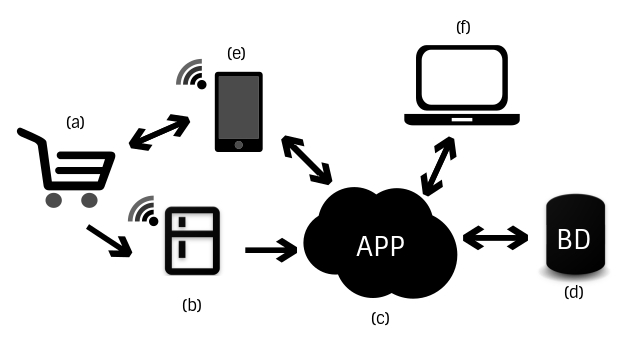
\includegraphics[width=16cm, height=8cm, scale=1]{./figures/architecture.png}
	\caption{Arquitetura Geral do Projeto}
	\label{project-general-architecture}
\end{figure}

Após uma ida às compras, os itens adquiridos, Figura \ref{project-general-architecture}(a), são armazenados nos seus respetivos locais, Figura \ref{project-general-architecture}(b). Como forma de automatizar a recolha de informação relativa quer aos artigos obtidos quer às suas caraterísticas, utilizam-se sensores. O uso destes só é possível caso os rótulos dos itens se encontrem em formato digital \textit{standard}, com \textit{tags} \acrfull{nfc} \cite{nfcforum:nfc} ou \acrfull{rfid} \cite{rfidinc:rfid}, e os locais de armazenamento contenham os respetivos leitores de \textit{tags}.

Ao guardar os artigos nos locais de armazenamento, os mesmos devem ser lidos pelos leitores, de forma a que a informação presente na \textit{tag} e o tipo de movimento (entrada ou saída) possam ser enviados para a API, Figura \ref{project-general-architecture}(c). Assim, estes dados são posteriormente tratados e armazenados de forma persistente na \acrfull{bd}, Figura \ref{project-general-architecture}(d). A API é responsável por retornar dados para as aplicações cliente, Figura \ref{project-general-architecture}(e, f). É no servidor que está presente o algoritmo de previsão de stocks utilizado para efetuar a previsão quanto à duração de cada um dos itens em stock.

No contexto da gestão de stocks assume-se a existência de duas formas de apresentação para os itens em stock: avulsos e embalados. Os primeiros são conservados em sistemas de arrumação identificados com \textit{tags} programáveis por \textit{smartphones}, \ref{project-general-architecture}(e). Os detalhes dos itens são especificados pelo utilizador e carregados para a \textit{tag}. Já os segundos contêm os seus rótulos digitais com o seu detalhe guardado pelos embaladores.\\

%
% Secção 3.2 Análise
%
\section{Análise}\label{sec32}

O sistema de gestão de stocks é composto por 2 blocos principais: o bloco do lado do cliente e o bloco do lado do servidor, que se relacionam. A representação destes blocos é apresentada na Figura \ref{project-layers-structure}. 

\begin{figure}[H]
	\centering
	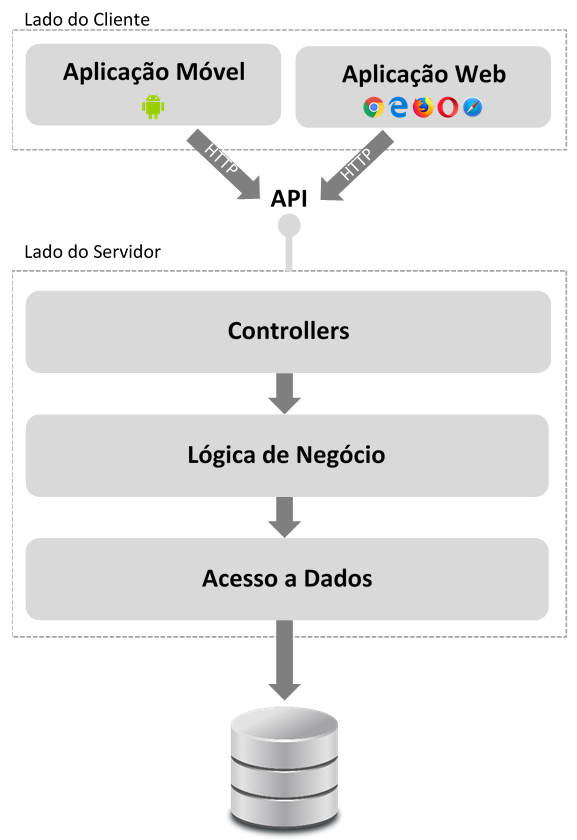
\includegraphics[height=9cm, scale=1]{./figures/project_architecture.png}
	\caption{Estrura por Camadas do Projeto}
	\label{project-layers-structure}
\end{figure}

O lado do servidor incluí três camadas e expõe uma \gls{api-web}. A \acrfull{dal} é produzida com a linguagem de programação \textit{Java}, usando a \acrfull{jpa}, e é responsável pelas leituras e escritas exercidas sobre a \acrfull{bd}. A \acrshort{bd} é externa ao servidor, utilizando para isso o \acrfull{sgbd} \textit{PostgreSQL}. A \acrfull{bll} é responsável pela aplicação das regras de negócio. A implementação desta camada é também realizada com linguagem \textit{Java}. Os \textit{controllers} foram desenvolvidos em \textit{Java} com a \textit{framework} da \textit{Spring}, chamada de \textit{Spring Boot}. A \gls{api-web} disponibiliza recursos em diferentes \textit{hypermedias}.

Do lado do cliente existem dois modos de interação, por uma aplicação móvel e outra por uma aplicação web. A aplicação móvel disponível para a plataforma \textit{Android}, desenvolvida em linguagem \textit{Kotlin}. A aplicação web é disponibilizada para a maioria dos browsers, e é implementada utilizando a linguagem \textit{JavaScript}, com o auxilio da \textit{framework Express}.